\documentclass[twocolumn]{ctexart}
% ctexart、ctexrep、ctexbook和ctexbeamer, 对应 LaTeX 的article、report、book和beamer
\usepackage[a4paper,left=2.5cm,right=2.5cm,top=2.6cm,bottom=2.6cm]{geometry} % 设置页面尺寸
\usepackage{fancyhdr} % 设置页眉页边页脚
\usepackage{multicol} % 多栏排版
\usepackage{xeCJK} % 中文支持
\usepackage{ctex} % 中文支持
\usepackage{footmisc} % 控制脚注格式,包括编号、字体、分隔线等
\usepackage{titletoc} % 定制目录列表样式
\usepackage{fontspec} % XeTeX下的字体选择宏包
\usepackage{setspace} % 行距
\usepackage{graphicx} % 插图
\usepackage{pdfpages} % 引用pdf页面
\usepackage{booktabs} % 三线表
\usepackage{multirow} % 表格多行支持
\usepackage{caption} % figure和table等中的说明文字
\usepackage{tikz} % 绘图
\usepackage{etoolbox} % 给宏包打补丁
\usepackage{hyperref} % 超链接
\usepackage{xcolor} % 颜色支持
\usepackage{array} % 数学表格
\usepackage{amsmath} % 数学公式
\usepackage{amssymb} % 数学字体与符号
\usepackage{amsthm} % 数学定理格式
\usepackage{subfig} % 排版子图
\usepackage{float} % 浮动体格式控制
\usepackage{lmodern} % 一种字体支持
\usepackage{listings} % 插入代码
\usepackage{tcolorbox} % 好看的块环境
\usepackage{pifont} % 字体支持
\usepackage{perpage} %the perpage package
\usepackage{mathdesign} % some math fonts
\usepackage{ulem} %一些文字强调的宏包
\usepackage{fancyvrb} % some fancy verbatim 
\usepackage{enumitem} % 列表项目
\usepackage{txfonts} % 一些字体
\usepackage{makecell}
\usepackage{mathrsfs}
\usepackage{subfig}                 % 子图包,不要与{subfigure}混用,{subfig}较新
\usepackage{overpic}   
%重置每页脚注序号
\pagestyle{headings}
\MakePerPage{footnote} %the perpage package command
\renewcommand \thefootnote{\ding{\numexpr171+\value{footnote}}}
% 为tcolorbox导入三个程序包
\tcbuselibrary{skins, breakable, theorems} 

% 设置代码格式 - 关键字加粗, 其余为正常。非彩色
\lstset{
    aboveskip=5mm,
    belowskip=5mm,
    breaklines=true,
    breakatwhitespace=true,
    columns=flexible,
    extendedchars=false,
    showstringspaces=false,
    numbers=none,
    basicstyle={\small\ttfamily},
    captionpos=t,
    frame=tb,
    tabsize=4
}

\lstdefinestyle{cpp} {
  language=C++
}

\lstdefinestyle{c++} {
  language=C++
}

\lstdefinestyle{python} {
  language=python,
  morekeywords={as}
}


% 为目录添加 PDF 链接
\addtocontents{toc}{\protect\hypersetup{hidelinks}}

% 设置「目录」二字格式
\renewcommand{\contentsname}{
  \fontsize{16pt}{\baselineskip}
  \normalfont\heiti{目~~~~录}
  \vspace{-8pt}
}

% 定理、定义、证明
\newtheorem{theorem}{定理}[section]
\newtheorem{definition}{定义}[section]
\newtheorem{lemma}{引理}[section]
\newtheorem{corollary}{推论}[section]
\newtheorem{example}{例}
\newtheorem{proposition}{命题}[section]

\title{机械设计基础突击}
\author{洛白}
\date{\today}

\begin{document}

% 显示标题作者时间
% \maketitle
% \newpage

% 调整目录行间距
% \renewcommand{\baselinestretch}{1.35}
% % 添加目录
% \tableofcontents
% \newpage

% 正文 22 磅的行距
\setlength{\parskip}{0em}
\renewcommand{\baselinestretch}{1.53}

\section{凸轮}
基圆半径(理论廓线最小)

凸轮的组成:从动件,凸轮,机架。

设计:反转法

\begin{description}[leftmargin=1.7cm,style=nextline,nosep]% nosep没有垂直间隔
  \item[理论廓线] 滚子中心,下面其他的定义都是基于理论廓线开始的。
  \item[偏置圆]
  \item[基圆]
  \item[推程] 从开始位置到最大位移位置
  \item[回程] 从最远位置到底最小位移位置 
  \item[压力角] 过廓线接触点 B 作法线 nn 与\textbf{从动件}的运动方向之间的夹角 α 就是其压力角 
          \begin{figure}[H]
              \centering
              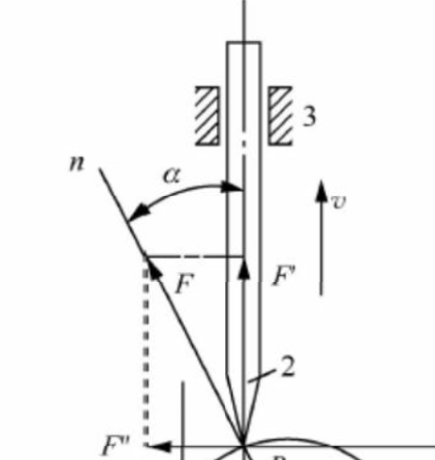
\includegraphics[width=5cm]{img/15.png}
              \end{figure}    
  \item[凸轮转角] 从初始位置,记得是做切线找。
  \item[位移] 位移怎么找来着????? 
  \item[最大位移]  
\end{description}

\begin{quote}
{\qquad\parindent2\ccwd\kaishu\zihao{5}
左偏置可以减小压力角。
}
\end{quote}

\subsection{不同的运动形式}
\begin{description}[leftmargin=1.7cm,style=nextline,nosep]% nosep没有垂直间隔
  \item[等速运动
  ]  刚性冲击
  \item[简谐运动] 柔性冲击,中低速。
  \item[正弦加速] 无突变,高速凸轮。 
\end{description}
\section{齿轮结构,轮系和齿轮传动}
本章节主要考点为齿轮机构的特点和类型,啮合基本定理,渐开线轮廓,部分名称和基本尺寸。渐开线尺寸的啮合和切齿原理,
定轴轮系传动笔计算和齿轮传动的失效形式,设计准则。强度??
圆柱齿轮传动的受力分析和强度计算。
\subsection{齿轮机构的特点和类型}
\subsection{特点}
\begin{description}[leftmargin=1.7cm,style=nextline,nosep]% nosep没有垂直间隔
    \item[传动比准确,传动平稳]
    \item[效率高] 大于$99\%$
\end{description}
主要是平面齿轮机构(柱)和空间齿轮机构(锥)。
\subsection{部分名称和基本尺寸}
        \begin{figure}[H]
            \centering
            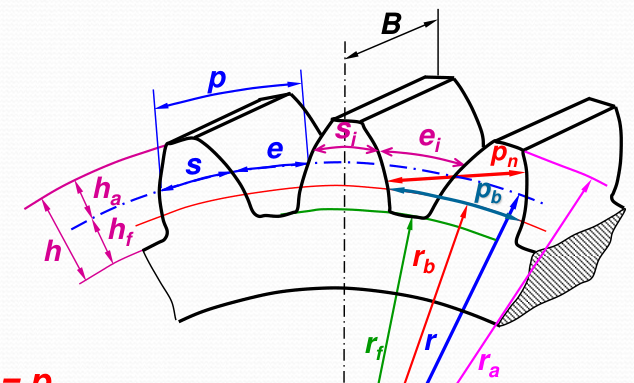
\includegraphics[width=7cm]{img/1.png}
            \end{figure}
\subsubsection{部分名称}
\begin{description}[leftmargin=1.5cm,style=nextline,nosep]% nosep没有垂直间隔
  \item[齿顶圆(above)] $d_a,r_a,h_a$
  \item[齿根圆] $r_f,d_f,h_f$
  \item[齿厚] $e_i$
  \item[齿槽宽] $s_i$
  \item[齿距] $p_i=e_i+s_i$
  \item[分度圆] $e_i=s_i$ 时候的圆,规定的计算基准圆  
  \item[齿全高] $h=h_a+h_f$
  \item[齿宽]$B$    
  \item[重合度] $\displaystyle \varepsilon =\frac{啮合弧}{齿矩}$    
\end{description}
\subsubsection{基本参数}
记住以下五个基本参数:齿数,模数,分度圆压力角,齿顶高系数,顶隙系数。注意中心距不是基本参数。
\begin{description}[nosep]% nosep没有垂直间隔
  \item[齿数] $Z$
  \item[模数] $m$ (mm)
  \begin{align}
    l=\pi d= p z &\implies d=\frac{p}{\pi}z\\
    m&=\frac{p}{m}
  \end{align}
  \item[分度圆压力角] $\alpha$ 渐开线某一点的速度方向(切线)和其受力(和原点连线垂线)。
          \begin{figure}[H]
              \centering
              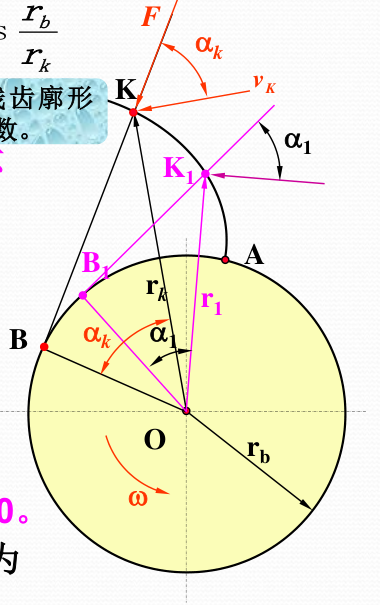
\includegraphics[width=4cm]{img/2.png}
              \end{figure}
  $$ \cos \alpha_k=\sin \angle{BKO}=\frac{BO}{BK}=\frac{r_b}{r_k} $$
  
  不同半径处$\alpha$ 还不一样。基,齿顶,分度圆的$r_k$ 分别为$r_b,r_a,r$
  \item[齿顶高系数] $h_a^*$
  \item[顶隙系数] $c^*$
\end{description}
\subsubsection{直齿轮主要计算公式}
        \begin{figure}[H]
            \centering
            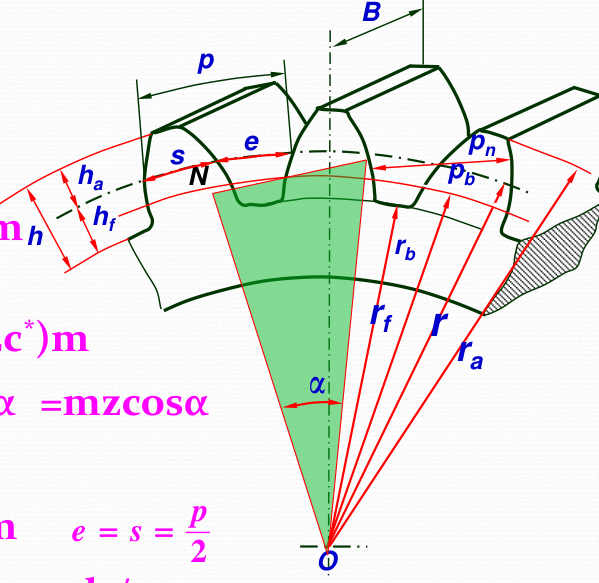
\includegraphics[width=6cm]{img/3.png}
            \end{figure}
\paragraph{对于直线:}
\begin{align*}
h_a&=h_a^*m\\
h_f&=(h_a*+c*)^*m\\
h&=h_a+h_f=(c^*+2h_a^*)\\
c&=c*m
\end{align*}

为什么规定齿根高要比齿顶高大呢?显然我不知道。

\textbf{并且对于正常齿,$1,0.25$。短,$0.8,0.3$。这个参数是你应该记住的,题目中有时候不会给出。你在算m的时候用的是分度圆的,但题目往往不会给出分度圆的。}


\paragraph{对于圆:}
\begin{description}[leftmargin=2.3cm,style=nextline,nosep]% nosep没有垂直间隔
  \item[分度圆直径] $d=mz$
  \item[齿顶圆直径] $d_a=d+2h_a=(z+2h_a^*)m$
  \item[齿根圆直径] $d_f=d\mathbf{-2h_f} =(z-2h_a^*-2c^*)m$  
  \item[基圆半径] $d_b=d\cos \alpha=mz\cos \alpha$ 
\end{description}

\paragraph{对于弧}
\begin{description}[leftmargin=2.3cm,style=nextline,nosep]% nosep没有垂直间隔
  \item[分度圆齿距] $m=\frac{p}{\pi}$
  \item[法向齿距] $p \cos \alpha$
\end{description}

\begin{quote}
{\qquad\parindent2\ccwd\kaishu\zihao{5}
对于内齿轮的话,$d_a=d-2h_a,d_f=d+2h_f$
}
\end{quote}

\begin{quote}
  {\qquad\parindent2\ccwd\kaishu\zihao{5}
  对于斜齿轮的话
  $$
  m_t=\frac{m_n}{\cos \beta}
  $$
  后面的用$m_t$来算就行
  }
  
\end{quote}
\paragraph{重要概念}
\begin{itemize}
\item 节圆的大小随中心距变化而变化。分度圆的大小只要齿轮加工好后就确定了
\item 分度圆的半径不能大于节圆的半径。
\item 分度圆:任一齿轮都有大小确定的分度圆。节圆:一对齿轮啮合时才存在,表明齿轮啮合特性
\end{itemize}

\subsection{渐开线尺寸的啮合和切齿原理}
\subsubsection{正确啮合条件}
\begin{align*}
  m_1&=m_2=m\\
\alpha_1&=\alpha_2=20
\end{align*}
\begin{description}[leftmargin=1.3cm,style=nextline,nosep]% nosep没有垂直间隔
  \item[正确啮合条件] $\alpha_{1}=\alpha_2=\alpha,m_1=m_2=m$ 
  \item[传动比] $n_{12}=\frac{d_2}{d_1}=\frac{z_2}{z_1}$ 
  \item[标准中心距] 分度圆相切时的中心距。当按标准中心距连接时
   $$
   a=r_1+r_2=\frac{m(z_1+z_2)}{2}
   $$
   \item[顶隙] $c=c*m=h_f-h_a$ 
   \item[连续传动] $\varepsilon >1$ 
\end{description}

\subsection{定轴轮系传动比}

\subsection{受力分析和强度计算}
下面简要介绍一些概念
\begin{description}[leftmargin=2.3cm,style=nextline,nosep]% nosep没有垂直间隔
  \item[开式传动] 外露、灰尘、易磨损,适低速。
  \item[闭式传动]  封闭、润滑、适重用。
  \item[硬齿面齿轮]
  \item[软齿面齿轮] 
  \item[低速轻载]  
  \item[中速中载] 
  \item[高速重载] 
\end{description}
\subsubsection{失效形式} 
5种失效形式:部位、原因、措施。轮齿的主要失效形式有 5 种:轮齿折断、齿面点蚀、面胶合、面磨损和面塑性变形
        \begin{figure}[H]
            \centering
            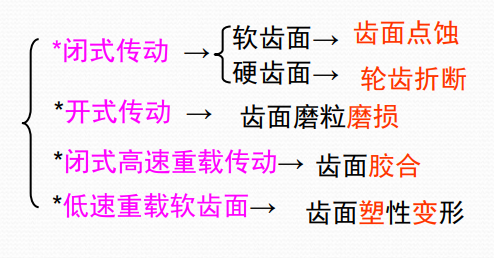
\includegraphics[width=6cm]{img/4.png}
            \end{figure}
\begin{description}[leftmargin=1.7cm,style=nextline,nosep]% nosep没有垂直间隔
  \item[轮齿折断]  一般发生在齿根部分,分过载折断和疲劳折断。其常见措施如下:
  \begin{description}[leftmargin=0.4cm,style=nextline,nosep]% nosep没有垂直间隔
    \item[1] 可以增大轴和支撑的刚度
    \item[2] 可以采用合适的热处理
    \item[3] 可以采用~,对齿根表面进行强化处理
    \item[4] 增大过度圆角半径,消除加工刀痕。   
  \end{description}
  \item[齿面点蚀]   载荷大,速度低,难以形成油膜。\textbf{主要闭式,开式不会有}。一般出现在齿根表面靠近节线处。
  \begin{quote}
  {\qquad\parindent2\ccwd\kaishu\zihao{5}
  可以提高强度和合理选择润滑油
  }
  \end{quote}
  \item[齿面胶合]   \textbf{高速重载、低速重载(冷胶合)闭式传动}的主要破坏形式。
  \begin{quote}
  {\qquad\parindent2\ccwd\kaishu\zihao{5}
  对于低俗可以增加润滑油粘度,对于高速可以加抗胶合添加剂。
  }
  \end{quote}
  \item[齿面磨损]    \begin{itemize}[nosep]
  \item \textnormal{磨粒磨损}是由于灰尘、硬屑粒等进入齿面间而引起的磨粒磨损。(\textbf{开式传动}容易发生)
  \item \textbf{跑合磨损}新机器。
  \end{itemize}
  \begin{quote}
  {\qquad\parindent2\ccwd\kaishu\zihao{5}
  可以增加齿面硬度,减小粗糙度,改善润滑环境,清洁环境。
  }
  \end{quote}
  \item[齿面塑性变形] 齿面沿摩擦力方向塑性变形
\end{description}
\subsection{模锻法切制法}
\subsubsection{仿形法(成形)}
\begin{quote}
{\qquad\parindent2\ccwd\kaishu\zihao{5}
在普通铣床上利用渐开线齿形的成形铣刀将齿坯齿槽部分的材料铣掉
}
\end{quote}
简单但是精度差,适用于单件生产。
\subsubsection{设计准则}
        \begin{figure}[H]
            \centering
            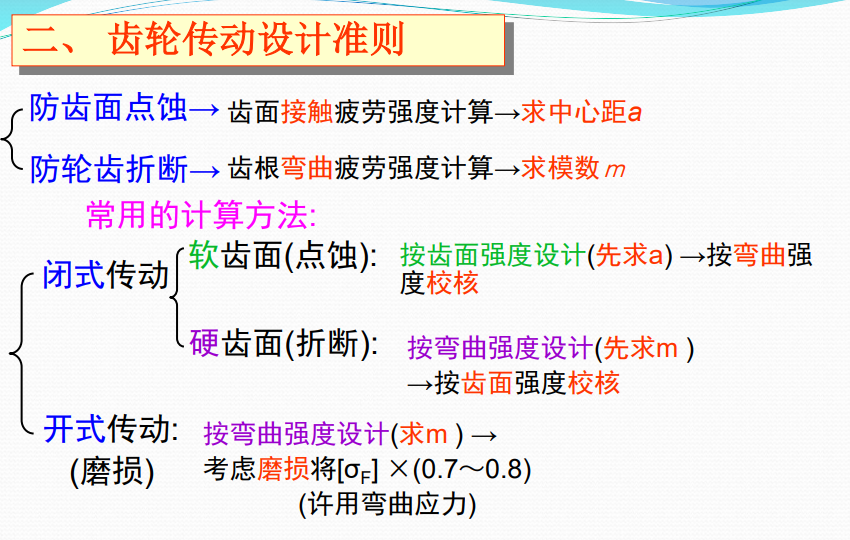
\includegraphics[width=8cm]{img/5.png}
            \end{figure}
\subsubsection{展成法(范成法或包络法)}
\begin{quote}
{\qquad\parindent2\ccwd\kaishu\zihao{5}
利用一对齿轮无侧隙啮合时两轮的齿廓互为包络线原理来加工齿形的一种加工方法。
}
\end{quote}
效率精度高,但是需要专门机床,可以批量生产。
\subsection{题目}
直齿圆柱外齿轮的基圆半径一定小于齿根圆直径。 ( 错)

满足啮合条件的一对齿轮一定连续传动。 (错 )

一对圆柱齿轮,在确定大小齿轮的宽度时,通常把小齿轮的齿宽做得比大齿轮的宽些其目的是:为便于安装,保证接触线的长度。(?)


轮系的传动比计算只需要计算传动比的大小即可。 (错)

两个齿轮的材料、齿宽、齿数相同,模数m,=2mm,m,=4mm,它们的弯曲强度承载能力,第二个比第个大提高齿面硬度可以提高齿轮抗折断能力.( )

采用合适的热处理方法提高轮芯韧性无法提高齿面抗点蚀的能聚真轴

轮系传动比计算中的转向关系判定都可以用“+、

闭式齿轮与开式齿轮的党见失效形式分别是什么?
\section{一些小题简答题}
\subsection{常见轴承类型(367N)及其受力特点,滚动轴承寿命计算}
\begin{quote}
{\qquad\parindent2\ccwd\kaishu\zihao{5}
按照受力分向心轴承和推力轴承。
}
\end{quote}
\begin{description}[leftmargin=2.8cm,style=nextline,nosep]% nosep没有垂直间隔
  \item[3 圆锥滚子轴承] 能同时承受较大的径向载荷和轴向载荷
  \item[6 深沟球轴承] 主要承受径向载荷,同时也可承受一定量的轴向载荷
  \item[7 角接触球轴承] 能同时承受径向、轴向\textbf{联合}载荷(高速支点?)
  \item[N 圆柱滚子轴承]  能承受较大的径向载荷,不能承受轴向载荷
  \item[5 推力球轴承] 
  \item[NA 滚针轴承] 
\end{description}
\begin{quote}
{\qquad\parindent2\ccwd\kaishu\zihao{5}
367N,追狗叫住
}
\end{quote}
\subsection{寿命}
\begin{description}[leftmargin=1.7cm,style=nextline,nosep]% nosep没有垂直间隔
  \item[轴承寿命] 轴承任一元件出现疲劳点蚀之前的总转数$(10^6r)$或者总工作小时$(h)$。
  \item[基本额定寿命 $L_{10}$]  一批相同轴承,其中百分之九十不出现疲劳点蚀之前的总转数$(10^6r)$或者总工作小时$(h)$。
   \item[基本额定动载荷] 轴承在基本额定寿命时所能承受的最大载荷。
   \item[当量动载荷]  对于向心轴承,C 为径向载荷Cr。对于推力轴承,C 为轴向载荷Ca。也有可能都承受。
\end{description}
        \begin{figure}[H]
            \centering
            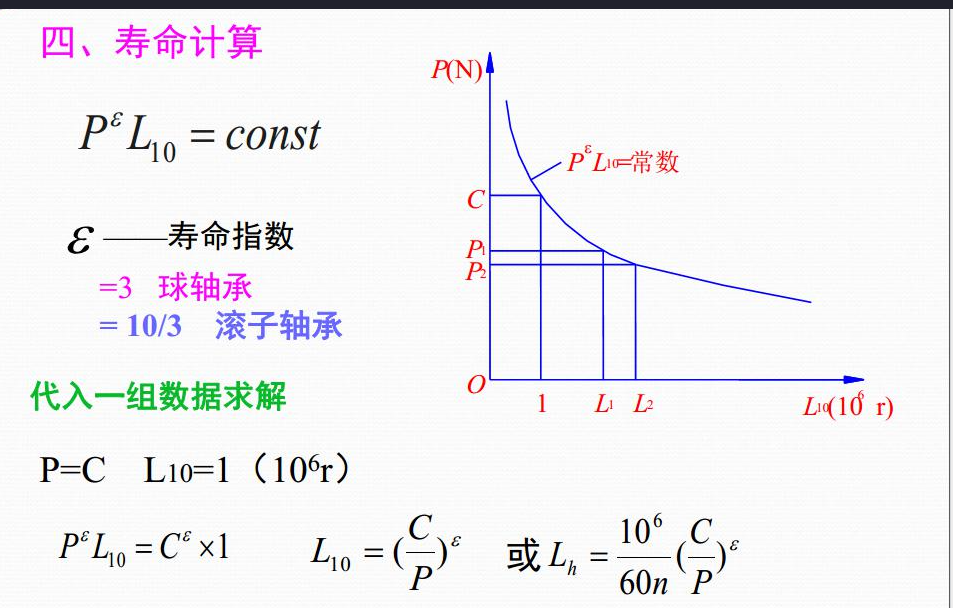
\includegraphics[width=8cm]{img/9.png}
            \end{figure}
$L_{10}$是多少转,$L_{h}$是多少小时。还可以引入温度系数$f_t$和动载荷系数$f_p$
$$ L_{h}= \frac{10^{6}}{60n}(\frac{f_{t}C}{f_{P}P})^{\varepsilon} $$
\begin{quote}
{\qquad\parindent2\ccwd\kaishu\zihao{5}
只有3,N是滚子轴承是$\displaystyle \frac{10}{3}$
}
        \begin{figure}[H]
            \centering
            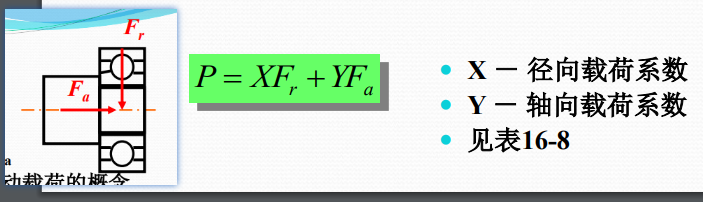
\includegraphics[width=8cm]{img/10.png}

            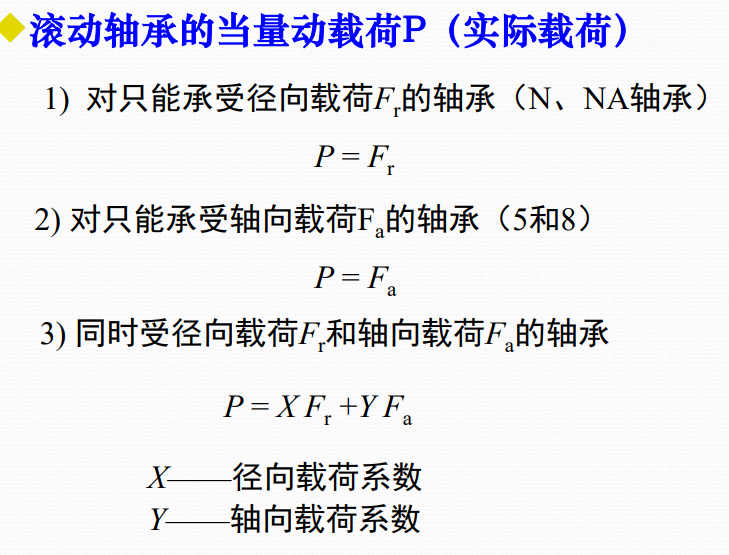
\includegraphics[width=8cm]{img/11.png}
          \end{figure}
\end{quote}

我们需要重点掌握的是如下的\textcolor{red}{\textbf{角接触向心轴承的实际轴向载荷}}!!!
        \begin{figure}[H]
            \centering
            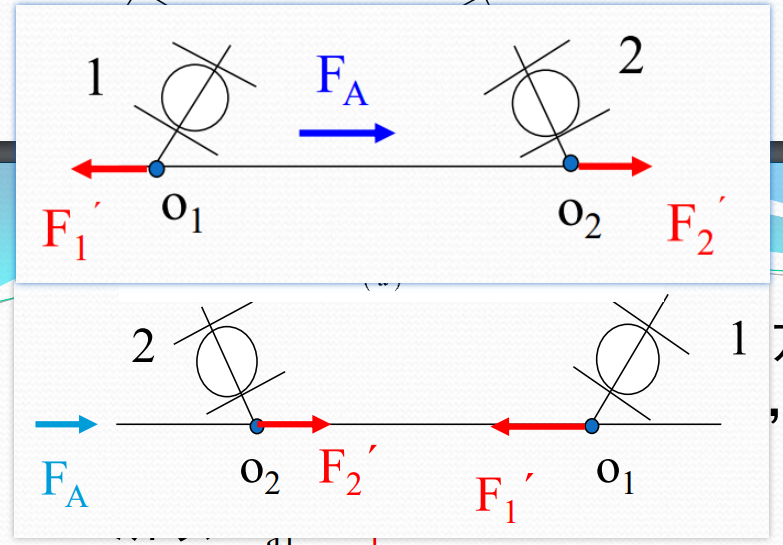
\includegraphics[width=7cm]{img/12.png}
            \end{figure}
小内正,大外反。或者箭头就是从交出的箭头方向。
        \begin{figure}[H]
            \centering
            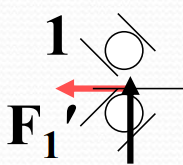
\includegraphics[width=5cm]{img/14.png}
            \end{figure}
先判断哪端压紧。放松端轴承的轴向载荷 = 内部轴向力,压紧端轴承的轴向载荷 = 除去本身内部轴向力后其余轴向
力的\textcolor{red}{\textbf{代数和}}(注意这个实时$F_1'$ 并不是$F_a$,,,)。并且有
$$
e=\frac{F_1'}{F_{r_1}}
$$
\begin{quote}
{\qquad\parindent2\ccwd\kaishu\zihao{5}
记得给出谁是危险轴承(2分),P大的那个之危险轴承。
}
\end{quote}
\begin{figure}[H]
            \centering
            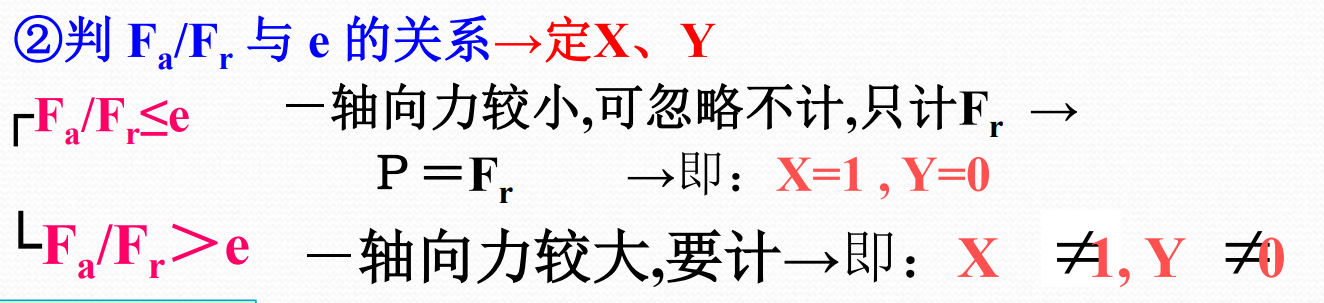
\includegraphics[width=8.5cm]{img/13.png}
            \end{figure}
            \begin{quote}
            {\qquad\parindent2\ccwd\kaishu\zihao{5}
            上面这个图是得出P的。
            }
            \end{quote}
\section{间歇运动机构}
\section{连接}
\subsection{螺纹连接}
\subsubsection{螺纹的主要参数}
        \begin{figure}[H]
            \centering
            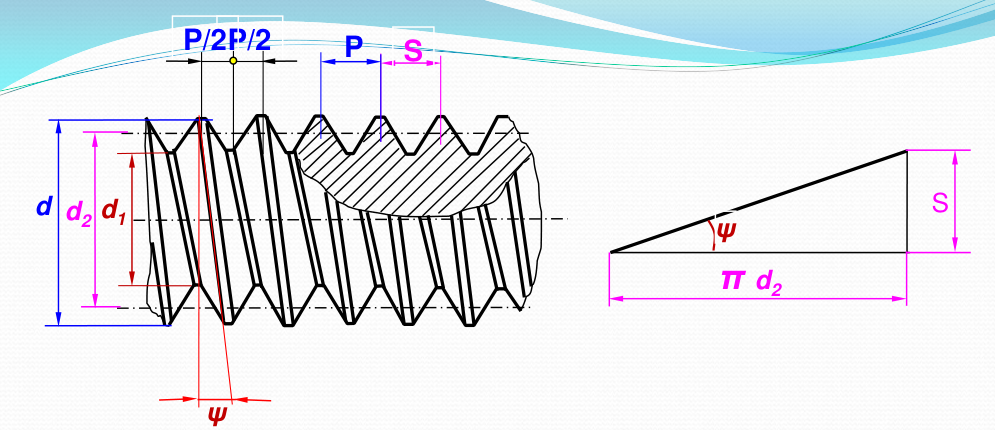
\includegraphics[width=8cm]{img/6.png}
            \end{figure}
            \begin{description}[leftmargin=1.7cm,style=nextline,nosep]% nosep没有垂直间隔
              \item[螺 距 P]  相邻两牙在中径线上对应两点间的轴向距离
              \item[导程 S] 同一螺旋线上相邻两牙在中径线上对应两点间的轴向距离
              \item[线数] 螺纹螺旋线数目,有
              $$
              S=np
              $$
              \item[螺纹升角] (普通螺纹是单线)
              $$ \tan \psi=\frac{S}{\pi d_2}=\frac{np}{\pi d_2}
              $$ 
                      \begin{figure}[H]
                          \centering
                          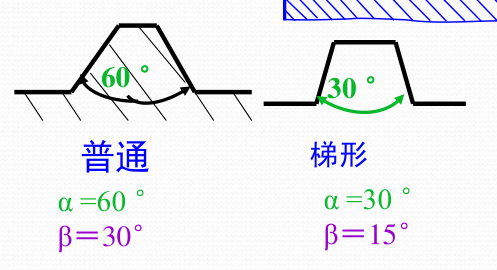
\includegraphics[width=7cm]{img/7.png}
                          \end{figure}
              \item[牙型角α] 螺纹轴向平面内螺纹牙型两侧边的夹角
              \item[牙侧角β] 螺纹牙的侧边与螺纹轴线垂直平面的夹角
            \end{description}
\subsection{螺栓联接的强度计算(!必考!)}
$$
[\sigma]=\frac{\sigma}{S}=\frac{\text{屈服极限}}{\text{安全系数}}
$$
\subsubsection{松螺栓}
$$
\sigma = \frac{F_{a}}{\pi d_{1}^{2}/4}\leq \left[ \sigma \right]
$$
这种情况只有起重机。
\subsubsection{紧螺栓}
对于其极限情况,也叫最大预紧力:
$$  \sigma _{v}= \frac{1.3F_0}{\pi d_{1}^{2}/4}= \frac{4 \times 1.3F_0}{\pi d_{1}^{2}}\leq \left[ \sigma \right] $$
对于一般
$$ F^{\prime}= \frac{KF_{R}}{fm} $$
\begin{description}[leftmargin=0.7cm,style=nextline,nosep]% nosep没有垂直间隔
  \item[f] 被连接件接合面之间的摩擦系数;
  \item[m] 被连接件接合面数目,图$ 11-15a $中,$ m=1 $,图$ 11-15b $中,$ m=2 $
  \item[K] 考虑摩擦传力的可靠系数,$ K=1.1 \sim 1.5 $。
   
\end{description}
        \begin{figure}[H]
            \centering
            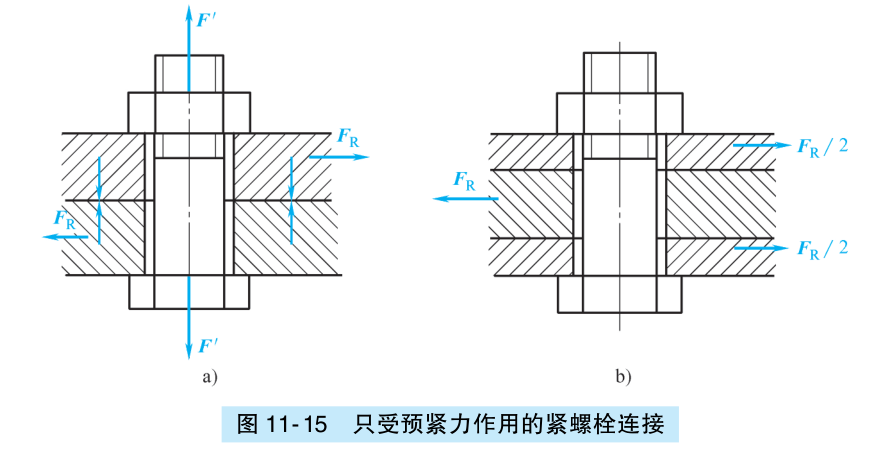
\includegraphics[width=8cm]{img/8.png}
            \end{figure}
剩余预紧力$(F'',F_R)$ 工作载荷 $(F,F_E)$
对于\textbf{最小轴向},有预紧力 $F_0$ (轴向拉力),总拉力$F_a$
$$ F_0=F_R+ \frac{k_{c}}{k_{c}+k_{b}}F_E $$
$$ F_a=F_0+ \frac{k_{b}}{k_{c}+k_{b}}F_E $$
上下两个一个是连接的相对刚度,一个是螺栓连接的相对刚度。
注意求总的预紧力用的是连接件的也就是1-螺栓连接的。显然就起来就有
$$
F_a =F_R+F_E
$$
$F_0$是预紧力,是最小轴向拉力。
\begin{quote}
{\qquad\parindent2\ccwd\kaishu\zihao{5}
0a,cb。注意1.3!!!!!!!
}
\end{quote}
\section{带传动}
\subsection{带传动的基本理论}
        \begin{figure}[H]
            \centering
            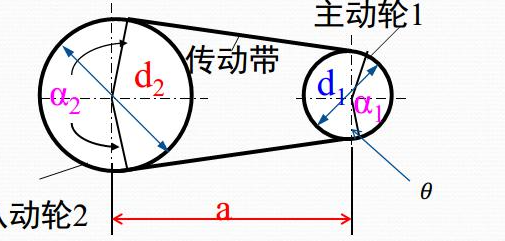
\includegraphics[width=7cm]{img/16.png}
            \end{figure}
基准长度
$$ L_{d}=2a+ \frac{\pi(d_{2}+d_{1})}{2}+ \frac{(d_{2}-d_{1})^{2}}{4a} $$

绕进主动轮的是紧边,绕出主动轮的是松边。紧边拉力$F_1$,松边$F_2$
\begin{align*}
F_1-F_0&=F_0-F_2\\
F_0&=\frac{1}{2}(F_1+F_2)\\
F_f&=F_1-F_2\\
F_1&=F_0+\frac{F_f}{2}\\
F_2&=F_0-\frac{F_f}{2}\\
P&=\frac{FV}{1000}
\end{align*}

$F_f>F_{\max}$ 的时候就打滑。在其刚要打滑的时候,有
$$
\frac{F_1}{F_2}=e^{f\alpha}
$$
带速
$$ v= \frac{\pi d_{1}n_{1}}{60 \times 1000}m/s $$

小带轮包角
$$  \alpha _{1}\approx 180^{\circ}- \frac{d_{d2}-d_{d1}}{a}\times 57.3^{\circ} $$
联立可以求解得到
$$\left\{ \begin{matrix}  F_{1}=F \frac{e^{f \alpha}}{e^{f_{\alpha}}-1}  \\  F_{2}=F \frac{1}{e^{f_{\alpha}}-1}  \\  F=F_{1}-F_{2}=F_{1}(1- \frac{1}{e^{f_{\alpha}}})  \end{matrix} \right.$$

\begin{quote}
{\qquad\parindent2\ccwd\kaishu\zihao{5}
增大包角,初拉力,摩擦力,都可以提高其所能传递的有效圆周力。
}
\end{quote}

\begin{description}[leftmargin=1.7cm,style=nextline,nosep]% nosep没有垂直间隔
  \item[弹性滑动] 弹性滑动不可避免。其是因带的弹性变化导致的带和带轮之间的相对运动。
  \item[打滑] 打滑可以避免,先发生在\textbf{小带轮}处  
\end{description}
        \begin{figure}[H]
            \centering
            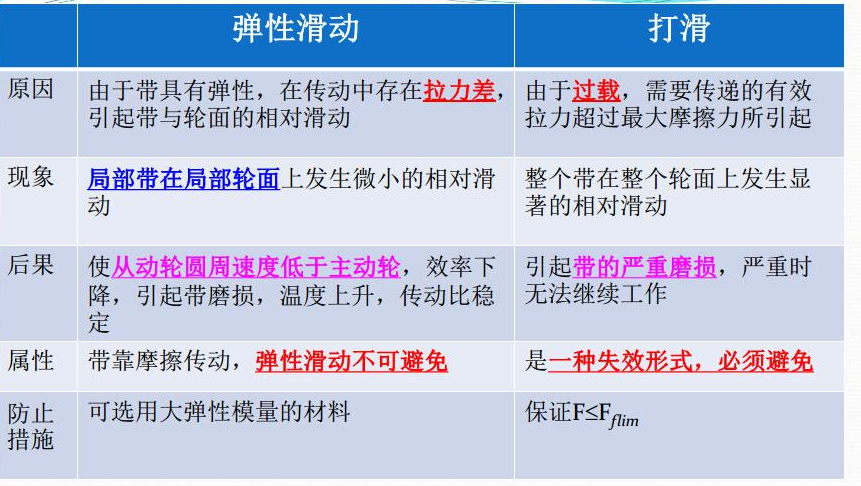
\includegraphics[width=8cm]{img/17.png}
            \end{figure}
避免打滑,可将带轮上与带接触的表面加工得粗糙些以增大摩擦(对)


在V带传动设计中,限制带得根数是为了使每根带受力不致太大。(对)


V带在减速传动过程中,带的最大应力应在\textbf{V带小带轮处}。(对)
带传动的中心距过小会使得带的寿命降低。(对)使得包角(\textbf{变小})

V带传动的弹性滑动可避免。(错)

减小V带传动的小带轮包角会降低带的工作能力()
在V带传动中,能提高传递得最大有效圆周力得影响因素有哪些?(包角,摩擦系数,初拉力)
(四种即可)
\section{连接}

\subsection{题目}
\paragraph{常用螺纹连接的类型有哪些?}
螺栓,螺钉,双头螺柱。
\paragraph{普通螺纹连接、双头螺柱连接和螺钉连接的应用场合分别是什么?}
        \begin{figure}[H]
            \centering
            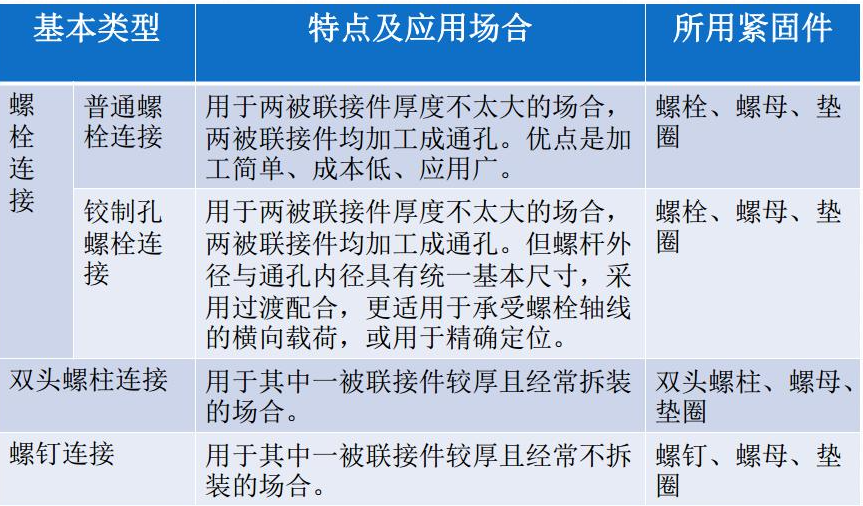
\includegraphics[width=7cm]{img/18.png}
            \end{figure}
\paragraph{半圆键的工艺性好,装拆方便。}(对对)
\paragraph{平键与半圆键都是靠键的两侧面来传递载荷。}(对)
\paragraph{平键连接能传递的最大扭矩为T,现要传递扭矩为1.5T,不改变键所在轴的直径和轮毂长度,则应安装一对平键。(对)}
\paragraph{键连接的四种主要类型?} 平键连接,半圆键连接,楔键连接,切向键连接。
\paragraph{根据用途不同,说出四种平键连接中的两种?}普通平键,导向平键。
\begin{quote}
{\qquad\parindent2\ccwd\kaishu\zihao{5}
承载能力不够时采用,按180°布置两个键。一对平键按1.5个键计算
}
\end{quote}
\section{轴}
\begin{quote}
{\qquad\parindent2\ccwd\kaishu\zihao{5}
按照\textbf{负载情况}来分,有转轴,心轴,传动轴。
\textbf{心弯,传转,转都行。}
}
\end{quote}
\subsection{轴的设计}
定位,固定。
\subsubsection{轴的组成}
        \begin{figure}[H]
            \centering
            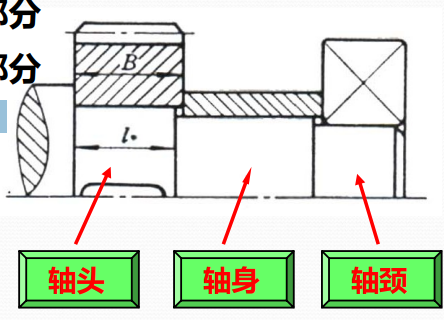
\includegraphics[width=7cm]{img/19.png}
            \end{figure}
\begin{description}[leftmargin=1.7cm,style=nextline,nosep]% nosep没有垂直间隔
  \item[轴头] 和旋转零件配合部分
  \item[轴身] 和轴承配合部分
  \item[轴颈] 连接轴头和轴身
  \item[轴肩]  轴的直径变
  化所形成的阶梯处
\end{description}
\section{联轴器和离轴器}
\end{document}